\documentclass[1p]{elsarticle_modified}
%\bibliographystyle{elsarticle-num}

%\usepackage[colorlinks]{hyperref}
%\usepackage{abbrmath_seonhwa} %\Abb, \Ascr, \Acal ,\Abf, \Afrak
\usepackage{amsfonts}
\usepackage{amssymb}
\usepackage{amsmath}
\usepackage{amsthm}
\usepackage{scalefnt}
\usepackage{amsbsy}
\usepackage{kotex}
\usepackage{caption}
\usepackage{subfig}
\usepackage{color}
\usepackage{graphicx}
\usepackage{xcolor} %% white, black, red, green, blue, cyan, magenta, yellow
\usepackage{float}
\usepackage{setspace}
\usepackage{hyperref}

\usepackage{tikz}
\usetikzlibrary{arrows}

\usepackage{multirow}
\usepackage{array} % fixed length table
\usepackage{hhline}

%%%%%%%%%%%%%%%%%%%%%
\makeatletter
\renewcommand*\env@matrix[1][\arraystretch]{%
	\edef\arraystretch{#1}%
	\hskip -\arraycolsep
	\let\@ifnextchar\new@ifnextchar
	\array{*\c@MaxMatrixCols c}}
\makeatother %https://tex.stackexchange.com/questions/14071/how-can-i-increase-the-line-spacing-in-a-matrix
%%%%%%%%%%%%%%%

\usepackage[normalem]{ulem}

\newcommand{\msout}[1]{\ifmmode\text{\sout{\ensuremath{#1}}}\else\sout{#1}\fi}
%SOURCE: \msout is \stkout macro in https://tex.stackexchange.com/questions/20609/strikeout-in-math-mode

\newcommand{\cancel}[1]{
	\ifmmode
	{\color{red}\msout{#1}}
	\else
	{\color{red}\sout{#1}}
	\fi
}

\newcommand{\add}[1]{
	{\color{blue}\uwave{#1}}
}

\newcommand{\replace}[2]{
	\ifmmode
	{\color{red}\msout{#1}}{\color{blue}\uwave{#2}}
	\else
	{\color{red}\sout{#1}}{\color{blue}\uwave{#2}}
	\fi
}

\newcommand{\Sol}{\mathcal{S}} %segment
\newcommand{\D}{D} %diagram
\newcommand{\A}{\mathcal{A}} %arc


%%%%%%%%%%%%%%%%%%%%%%%%%%%%%5 test

\def\sl{\operatorname{\textup{SL}}(2,\Cbb)}
\def\psl{\operatorname{\textup{PSL}}(2,\Cbb)}
\def\quan{\mkern 1mu \triangleright \mkern 1mu}

\theoremstyle{definition}
\newtheorem{thm}{Theorem}[section]
\newtheorem{prop}[thm]{Proposition}
\newtheorem{lem}[thm]{Lemma}
\newtheorem{ques}[thm]{Question}
\newtheorem{cor}[thm]{Corollary}
\newtheorem{defn}[thm]{Definition}
\newtheorem{exam}[thm]{Example}
\newtheorem{rmk}[thm]{Remark}
\newtheorem{alg}[thm]{Algorithm}

\newcommand{\I}{\sqrt{-1}}
\begin{document}

%\begin{frontmatter}
%
%\title{Boundary parabolic representations of knots up to 8 crossings}
%
%%% Group authors per affiliation:
%\author{Yunhi Cho} 
%\address{Department of Mathematics, University of Seoul, Seoul, Korea}
%\ead{yhcho@uos.ac.kr}
%
%
%\author{Seonhwa Kim} %\fnref{s_kim}}
%\address{Center for Geometry and Physics, Institute for Basic Science, Pohang, 37673, Korea}
%\ead{ryeona17@ibs.re.kr}
%
%\author{Hyuk Kim}
%\address{Department of Mathematical Sciences, Seoul National University, Seoul 08826, Korea}
%\ead{hyukkim@snu.ac.kr}
%
%\author{Seokbeom Yoon}
%\address{Department of Mathematical Sciences, Seoul National University, Seoul, 08826,  Korea}
%\ead{sbyoon15@snu.ac.kr}
%
%\begin{abstract}
%We find all boundary parabolic representation of knots up to 8 crossings.
%
%\end{abstract}
%\begin{keyword}
%    \MSC[2010] 57M25 
%\end{keyword}
%
%\end{frontmatter}

%\linenumbers
%\tableofcontents
%
\newcommand\colored[1]{\textcolor{white}{\rule[-0.35ex]{0.8em}{1.4ex}}\kern-0.8em\color{red} #1}%
%\newcommand\colored[1]{\textcolor{white}{ #1}\kern-2.17ex	\textcolor{white}{ #1}\kern-1.81ex	\textcolor{white}{ #1}\kern-2.15ex\color{red}#1	}

{\Large $\underline{12a_{0008}~(K12a_{0008})}$}

\setlength{\tabcolsep}{10pt}
\renewcommand{\arraystretch}{1.6}
\vspace{1cm}\begin{tabular}{m{100pt}>{\centering\arraybackslash}m{274pt}}
\multirow{5}{120pt}{
	\centering
	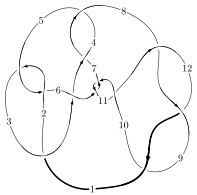
\includegraphics[width=112pt]{../../../GIT/diagram.site/Diagrams/png/809_12a_0008.png}\\
\ \ \ A knot diagram\footnotemark}&
\allowdisplaybreaks
\textbf{Linearized knot diagam} \\
\cline{2-2}
 &
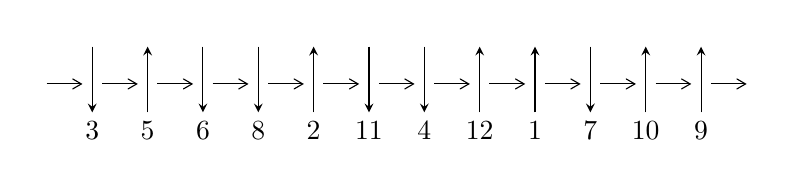
\begin{tikzpicture}[x=20pt, y=17pt]
	% nodes
	\node (C0) at (0, 0) {};
	\node (C1) at (1, 0) {};
	\node (C1U) at (1, +1) {};
	\node (C1D) at (1, -1) {3};

	\node (C2) at (2, 0) {};
	\node (C2U) at (2, +1) {};
	\node (C2D) at (2, -1) {5};

	\node (C3) at (3, 0) {};
	\node (C3U) at (3, +1) {};
	\node (C3D) at (3, -1) {6};

	\node (C4) at (4, 0) {};
	\node (C4U) at (4, +1) {};
	\node (C4D) at (4, -1) {8};

	\node (C5) at (5, 0) {};
	\node (C5U) at (5, +1) {};
	\node (C5D) at (5, -1) {2};

	\node (C6) at (6, 0) {};
	\node (C6U) at (6, +1) {};
	\node (C6D) at (6, -1) {11};

	\node (C7) at (7, 0) {};
	\node (C7U) at (7, +1) {};
	\node (C7D) at (7, -1) {4};

	\node (C8) at (8, 0) {};
	\node (C8U) at (8, +1) {};
	\node (C8D) at (8, -1) {12};

	\node (C9) at (9, 0) {};
	\node (C9U) at (9, +1) {};
	\node (C9D) at (9, -1) {1};

	\node (C10) at (10, 0) {};
	\node (C10U) at (10, +1) {};
	\node (C10D) at (10, -1) {7};

	\node (C11) at (11, 0) {};
	\node (C11U) at (11, +1) {};
	\node (C11D) at (11, -1) {10};

	\node (C12) at (12, 0) {};
	\node (C12U) at (12, +1) {};
	\node (C12D) at (12, -1) {9};
	\node (C13) at (13, 0) {};

	% arrows
	\draw[->,>={angle 60}]
	(C0) edge (C1) (C1) edge (C2) (C2) edge (C3) (C3) edge (C4) (C4) edge (C5) (C5) edge (C6) (C6) edge (C7) (C7) edge (C8) (C8) edge (C9) (C9) edge (C10) (C10) edge (C11) (C11) edge (C12) (C12) edge (C13) ;	\draw[->,>=stealth]
	(C1U) edge (C1D) (C2D) edge (C2U) (C3U) edge (C3D) (C4U) edge (C4D) (C5D) edge (C5U) (C6U) edge (C6D) (C7U) edge (C7D) (C8D) edge (C8U) (C9D) edge (C9U) (C10U) edge (C10D) (C11D) edge (C11U) (C12D) edge (C12U) ;
	\end{tikzpicture} \\
\hhline{~~} \\& 
\textbf{Solving Sequence} \\ \cline{2-2} 
 &
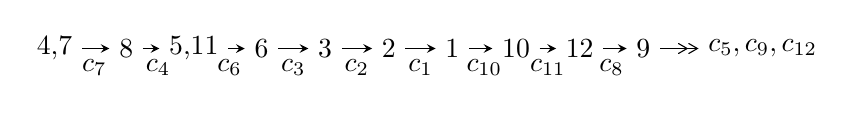
\begin{tikzpicture}[x=23pt, y=7pt]
	% node
	\node (A0) at (-1/8, 0) {4,7};
	\node (A1) at (1, 0) {8};
	\node (A2) at (33/16, 0) {5,11};
	\node (A3) at (25/8, 0) {6};
	\node (A4) at (33/8, 0) {3};
	\node (A5) at (41/8, 0) {2};
	\node (A6) at (49/8, 0) {1};
	\node (A7) at (57/8, 0) {10};
	\node (A8) at (65/8, 0) {12};
	\node (A9) at (73/8, 0) {9};
	\node (C1) at (1/2, -1) {$c_{7}$};
	\node (C2) at (3/2, -1) {$c_{4}$};
	\node (C3) at (21/8, -1) {$c_{6}$};
	\node (C4) at (29/8, -1) {$c_{3}$};
	\node (C5) at (37/8, -1) {$c_{2}$};
	\node (C6) at (45/8, -1) {$c_{1}$};
	\node (C7) at (53/8, -1) {$c_{10}$};
	\node (C8) at (61/8, -1) {$c_{11}$};
	\node (C9) at (69/8, -1) {$c_{8}$};
	\node (A10) at (11, 0) {$c_{5},c_{9},c_{12}$};

	% edge
	\draw[->,>=stealth]	
	(A0) edge (A1) (A1) edge (A2) (A2) edge (A3) (A3) edge (A4) (A4) edge (A5) (A5) edge (A6) (A6) edge (A7) (A7) edge (A8) (A8) edge (A9) ;
	\draw[->>,>={angle 60}]	
	(A9) edge (A10);
\end{tikzpicture} \\ 

\end{tabular} \\

\footnotetext{
The image of knot diagram is generated by the software ``\textbf{Draw programme}" developed by Andrew Bartholomew(\url{http://www.layer8.co.uk/maths/draw/index.htm\#Running-draw}), where we modified some parts for our purpose(\url{https://github.com/CATsTAILs/LinksPainter}).
}\phantom \\ \newline 
\centering \textbf{Ideals for irreducible components\footnotemark of $X_{\text{par}}$} 
 
\begin{align*}
I^u_{1}&=\langle 
-3.82254\times10^{339} u^{104}-5.03783\times10^{339} u^{103}+\cdots+5.84724\times10^{339} b-5.55902\times10^{342},\\
\phantom{I^u_{1}}&\phantom{= \langle  }1.82294\times10^{340} u^{104}+2.22909\times10^{340} u^{103}+\cdots+2.33889\times10^{340} a+2.44212\times10^{343},\\
\phantom{I^u_{1}}&\phantom{= \langle  }u^{105}+2 u^{104}+\cdots+2048 u+1024\rangle \\
I^u_{2}&=\langle 
b,\;- u^4+2 u^3+u^2+a-3 u,\;u^5- u^4-2 u^3+u^2+u+1\rangle \\
\\
I^v_{1}&=\langle 
a,\;-152 v^9+36 v^8-216 v^7+881 v^6-468 v^5+684 v^4-1376 v^3+252 v^2+115 b-144 v+219,\\
\phantom{I^v_{1}}&\phantom{= \langle  }v^{10}- v^9+2 v^8-7 v^7+8 v^6-9 v^5+14 v^4-10 v^3+5 v^2-3 v+1\rangle \\
\end{align*}
\raggedright * 3 irreducible components of $\dim_{\mathbb{C}}=0$, with total 120 representations.\\
\footnotetext{All coefficients of polynomials are rational numbers. But the coefficients are sometimes approximated in decimal forms when there is not enough margin.}
\newpage
\renewcommand{\arraystretch}{1}
\centering \section*{I. $I^u_{1}= \langle -3.82\times10^{339} u^{104}-5.04\times10^{339} u^{103}+\cdots+5.85\times10^{339} b-5.56\times10^{342},\;1.82\times10^{340} u^{104}+2.23\times10^{340} u^{103}+\cdots+2.34\times10^{340} a+2.44\times10^{343},\;u^{105}+2 u^{104}+\cdots+2048 u+1024 \rangle$}
\flushleft \textbf{(i) Arc colorings}\\
\begin{tabular}{m{7pt} m{180pt} m{7pt} m{180pt} }
\flushright $a_{4}=$&$\begin{pmatrix}0\\u\end{pmatrix}$ \\
\flushright $a_{7}=$&$\begin{pmatrix}1\\0\end{pmatrix}$ \\
\flushright $a_{8}=$&$\begin{pmatrix}1\\u^2\end{pmatrix}$ \\
\flushright $a_{5}=$&$\begin{pmatrix}- u\\- u^3+u\end{pmatrix}$ \\
\flushright $a_{11}=$&$\begin{pmatrix}-0.779404 u^{104}-0.953053 u^{103}+\cdots-752.424 u-1044.13\\0.653735 u^{104}+0.861575 u^{103}+\cdots+591.500 u+950.710\end{pmatrix}$ \\
\flushright $a_{6}=$&$\begin{pmatrix}1.76035 u^{104}+1.98543 u^{103}+\cdots+1749.68 u+2063.65\\-0.847121 u^{104}-1.09653 u^{103}+\cdots-781.787 u-1191.48\end{pmatrix}$ \\
\flushright $a_{3}=$&$\begin{pmatrix}0.959231 u^{104}+1.22999 u^{103}+\cdots+905.222 u+1333.17\\-1.35472 u^{104}-1.62405 u^{103}+\cdots-1278.29 u-1734.35\end{pmatrix}$ \\
\flushright $a_{2}=$&$\begin{pmatrix}1.51533 u^{104}+1.88583 u^{103}+\cdots+1422.48 u+2030.46\\-1.52651 u^{104}-1.83959 u^{103}+\cdots-1430.38 u-1964.33\end{pmatrix}$ \\
\flushright $a_{1}=$&$\begin{pmatrix}-0.913226 u^{104}-0.888902 u^{103}+\cdots-967.888 u-872.162\\-1.79713 u^{104}-2.06159 u^{103}+\cdots-1766.75 u-2151.53\end{pmatrix}$ \\
\flushright $a_{10}=$&$\begin{pmatrix}-0.125669 u^{104}-0.0914777 u^{103}+\cdots-160.924 u-93.4241\\0.653735 u^{104}+0.861575 u^{103}+\cdots+591.500 u+950.710\end{pmatrix}$ \\
\flushright $a_{12}=$&$\begin{pmatrix}-1.50997 u^{104}-1.64956 u^{103}+\cdots-1556.56 u-1732.04\\-0.184220 u^{104}-0.158133 u^{103}+\cdots-191.728 u-159.602\end{pmatrix}$ \\
\flushright $a_{9}=$&$\begin{pmatrix}-0.561315 u^{104}-0.724978 u^{103}+\cdots-476.369 u-771.780\\1.00686 u^{104}+1.15100 u^{103}+\cdots+1010.56 u+1206.98\end{pmatrix}$\\&\end{tabular}
\flushleft \textbf{(ii) Obstruction class $= -1$}\\~\\
\flushleft \textbf{(iii) Cusp Shapes $= -1.68427 u^{104}-1.92328 u^{103}+\cdots-1794.45 u-2081.91$}\\~\\
\newpage\renewcommand{\arraystretch}{1}
\flushleft \textbf{(iv) u-Polynomials at the component}\newline \\
\begin{tabular}{m{50pt}|m{274pt}}
Crossings & \hspace{64pt}u-Polynomials at each crossing \\
\hline $$\begin{aligned}c_{1}\end{aligned}$$&$\begin{aligned}
&u^{105}+53 u^{104}+\cdots-7 u-1
\end{aligned}$\\
\hline $$\begin{aligned}c_{2},c_{5}\end{aligned}$$&$\begin{aligned}
&u^{105}+7 u^{104}+\cdots+7 u+1
\end{aligned}$\\
\hline $$\begin{aligned}c_{3}\end{aligned}$$&$\begin{aligned}
&u^{105}-7 u^{104}+\cdots+40669 u+23377
\end{aligned}$\\
\hline $$\begin{aligned}c_{4},c_{7}\end{aligned}$$&$\begin{aligned}
&u^{105}+2 u^{104}+\cdots+2048 u+1024
\end{aligned}$\\
\hline $$\begin{aligned}c_{6},c_{10}\end{aligned}$$&$\begin{aligned}
&u^{105}+3 u^{104}+\cdots+96 u+32
\end{aligned}$\\
\hline $$\begin{aligned}c_{8},c_{9},c_{12}\end{aligned}$$&$\begin{aligned}
&u^{105}+8 u^{104}+\cdots+2 u+1
\end{aligned}$\\
\hline $$\begin{aligned}c_{11}\end{aligned}$$&$\begin{aligned}
&u^{105}-39 u^{104}+\cdots-14848 u+1024
\end{aligned}$\\
\hline
\end{tabular}\\~\\
\newpage\renewcommand{\arraystretch}{1}
\flushleft \textbf{(v) Riley Polynomials at the component}\newline \\
\begin{tabular}{m{50pt}|m{274pt}}
Crossings & \hspace{64pt}Riley Polynomials at each crossing \\
\hline $$\begin{aligned}c_{1}\end{aligned}$$&$\begin{aligned}
&y^{105}+5 y^{104}+\cdots-47 y-1
\end{aligned}$\\
\hline $$\begin{aligned}c_{2},c_{5}\end{aligned}$$&$\begin{aligned}
&y^{105}+53 y^{104}+\cdots-7 y-1
\end{aligned}$\\
\hline $$\begin{aligned}c_{3}\end{aligned}$$&$\begin{aligned}
&y^{105}-43 y^{104}+\cdots+5130220969 y-546484129
\end{aligned}$\\
\hline $$\begin{aligned}c_{4},c_{7}\end{aligned}$$&$\begin{aligned}
&y^{105}-60 y^{104}+\cdots+25165824 y-1048576
\end{aligned}$\\
\hline $$\begin{aligned}c_{6},c_{10}\end{aligned}$$&$\begin{aligned}
&y^{105}+39 y^{104}+\cdots-14848 y-1024
\end{aligned}$\\
\hline $$\begin{aligned}c_{8},c_{9},c_{12}\end{aligned}$$&$\begin{aligned}
&y^{105}-90 y^{104}+\cdots-206 y-1
\end{aligned}$\\
\hline $$\begin{aligned}c_{11}\end{aligned}$$&$\begin{aligned}
&y^{105}+47 y^{104}+\cdots-210108416 y-1048576
\end{aligned}$\\
\hline
\end{tabular}\\~\\
\newpage\flushleft \textbf{(vi) Complex Volumes and Cusp Shapes}
$$\begin{array}{c|c|c}  
\text{Solutions to }I^u_{1}& \I (\text{vol} + \sqrt{-1}CS) & \text{Cusp shape}\\
 \hline 
\begin{aligned}
u &= \phantom{-}0.966623 + 0.262000 I \\
a &= \phantom{-}1.84206 - 0.44039 I \\
b &= \phantom{-}0.613331 + 0.897632 I\end{aligned}
 & -0.62620 - 5.04939 I & \phantom{-0.000000 } 0 \\ \hline\begin{aligned}
u &= \phantom{-}0.966623 - 0.262000 I \\
a &= \phantom{-}1.84206 + 0.44039 I \\
b &= \phantom{-}0.613331 - 0.897632 I\end{aligned}
 & -0.62620 + 5.04939 I & \phantom{-0.000000 } 0 \\ \hline\begin{aligned}
u &= -0.994592 + 0.126675 I \\
a &= -0.11789 + 1.79257 I \\
b &= -0.244604 - 1.112200 I\end{aligned}
 & -1.41343 + 1.12338 I & \phantom{-0.000000 } 0 \\ \hline\begin{aligned}
u &= -0.994592 - 0.126675 I \\
a &= -0.11789 - 1.79257 I \\
b &= -0.244604 + 1.112200 I\end{aligned}
 & -1.41343 - 1.12338 I & \phantom{-0.000000 } 0 \\ \hline\begin{aligned}
u &= -0.156135 + 0.971665 I \\
a &= \phantom{-}0.04677 - 1.83355 I \\
b &= \phantom{-}0.595883 + 0.703683 I\end{aligned}
 & \phantom{-}0.09747 - 2.29231 I & \phantom{-0.000000 } 0 \\ \hline\begin{aligned}
u &= -0.156135 - 0.971665 I \\
a &= \phantom{-}0.04677 + 1.83355 I \\
b &= \phantom{-}0.595883 - 0.703683 I\end{aligned}
 & \phantom{-}0.09747 + 2.29231 I & \phantom{-0.000000 } 0 \\ \hline\begin{aligned}
u &= \phantom{-}0.996817 + 0.231114 I \\
a &= -0.119338 - 0.216906 I \\
b &= \phantom{-}1.148970 + 0.105590 I\end{aligned}
 & \phantom{-}0.82031 - 3.49410 I & \phantom{-0.000000 } 0 \\ \hline\begin{aligned}
u &= \phantom{-}0.996817 - 0.231114 I \\
a &= -0.119338 + 0.216906 I \\
b &= \phantom{-}1.148970 - 0.105590 I\end{aligned}
 & \phantom{-}0.82031 + 3.49410 I & \phantom{-0.000000 } 0 \\ \hline\begin{aligned}
u &= \phantom{-}0.830770 + 0.624559 I \\
a &= \phantom{-}0.50740 - 1.47941 I \\
b &= \phantom{-}0.195587 + 1.292660 I\end{aligned}
 & \phantom{-}8.20664 - 3.74731 I & \phantom{-0.000000 } 0 \\ \hline\begin{aligned}
u &= \phantom{-}0.830770 - 0.624559 I \\
a &= \phantom{-}0.50740 + 1.47941 I \\
b &= \phantom{-}0.195587 - 1.292660 I\end{aligned}
 & \phantom{-}8.20664 + 3.74731 I & \phantom{-0.000000 } 0\\
 \hline 
 \end{array}$$\newpage$$\begin{array}{c|c|c}  
\text{Solutions to }I^u_{1}& \I (\text{vol} + \sqrt{-1}CS) & \text{Cusp shape}\\
 \hline 
\begin{aligned}
u &= -1.06842\phantom{ +0.000000I} \\
a &= -0.124114\phantom{ +0.000000I} \\
b &= -0.549124\phantom{ +0.000000I}\end{aligned}
 & -1.78436\phantom{ +0.000000I} & \phantom{-0.000000 } 0 \\ \hline\begin{aligned}
u &= \phantom{-}0.289155 + 1.029210 I \\
a &= \phantom{-}0.010911 - 1.335340 I \\
b &= \phantom{-}0.859812 + 0.584753 I\end{aligned}
 & \phantom{-}0.42759 + 4.73730 I & \phantom{-0.000000 } 0 \\ \hline\begin{aligned}
u &= \phantom{-}0.289155 - 1.029210 I \\
a &= \phantom{-}0.010911 + 1.335340 I \\
b &= \phantom{-}0.859812 - 0.584753 I\end{aligned}
 & \phantom{-}0.42759 - 4.73730 I & \phantom{-0.000000 } 0 \\ \hline\begin{aligned}
u &= -0.765537 + 0.753961 I \\
a &= \phantom{-}1.22243 + 0.93816 I \\
b &= -0.075655 - 1.140690 I\end{aligned}
 & \phantom{-}6.95108 - 3.58416 I & \phantom{-0.000000 } 0 \\ \hline\begin{aligned}
u &= -0.765537 - 0.753961 I \\
a &= \phantom{-}1.22243 - 0.93816 I \\
b &= -0.075655 + 1.140690 I\end{aligned}
 & \phantom{-}6.95108 + 3.58416 I & \phantom{-0.000000 } 0 \\ \hline\begin{aligned}
u &= \phantom{-}0.298691 + 1.037650 I \\
a &= -0.200218 + 1.183490 I \\
b &= \phantom{-}0.621372 - 1.078950 I\end{aligned}
 & \phantom{-}4.62024 + 5.96188 I & \phantom{-0.000000 } 0 \\ \hline\begin{aligned}
u &= \phantom{-}0.298691 - 1.037650 I \\
a &= -0.200218 - 1.183490 I \\
b &= \phantom{-}0.621372 + 1.078950 I\end{aligned}
 & \phantom{-}4.62024 - 5.96188 I & \phantom{-0.000000 } 0 \\ \hline\begin{aligned}
u &= -0.915190 + 0.048307 I \\
a &= \phantom{-}1.57055 - 0.49914 I \\
b &= \phantom{-}0.606566 - 0.808414 I\end{aligned}
 & -0.915909 - 0.241093 I & \phantom{-0.000000 } 0 \\ \hline\begin{aligned}
u &= -0.915190 - 0.048307 I \\
a &= \phantom{-}1.57055 + 0.49914 I \\
b &= \phantom{-}0.606566 + 0.808414 I\end{aligned}
 & -0.915909 + 0.241093 I & \phantom{-0.000000 } 0 \\ \hline\begin{aligned}
u &= -0.951368 + 0.522622 I \\
a &= \phantom{-}0.38217 + 1.61581 I \\
b &= \phantom{-}0.252648 - 1.368440 I\end{aligned}
 & \phantom{-}6.29716 + 8.47800 I & \phantom{-0.000000 } 0\\
 \hline 
 \end{array}$$\newpage$$\begin{array}{c|c|c}  
\text{Solutions to }I^u_{1}& \I (\text{vol} + \sqrt{-1}CS) & \text{Cusp shape}\\
 \hline 
\begin{aligned}
u &= -0.951368 - 0.522622 I \\
a &= \phantom{-}0.38217 - 1.61581 I \\
b &= \phantom{-}0.252648 + 1.368440 I\end{aligned}
 & \phantom{-}6.29716 - 8.47800 I & \phantom{-0.000000 } 0 \\ \hline\begin{aligned}
u &= \phantom{-}0.771518 + 0.768489 I \\
a &= \phantom{-}0.94253 - 1.18145 I \\
b &= \phantom{-}0.017151 + 1.183720 I\end{aligned}
 & \phantom{-}8.47050 - 1.50689 I & \phantom{-0.000000 } 0 \\ \hline\begin{aligned}
u &= \phantom{-}0.771518 - 0.768489 I \\
a &= \phantom{-}0.94253 + 1.18145 I \\
b &= \phantom{-}0.017151 - 1.183720 I\end{aligned}
 & \phantom{-}8.47050 + 1.50689 I & \phantom{-0.000000 } 0 \\ \hline\begin{aligned}
u &= -1.075900 + 0.190627 I \\
a &= -1.365470 + 0.159370 I \\
b &= -0.603761 + 1.042000 I\end{aligned}
 & \phantom{-}3.68939 + 3.33964 I & \phantom{-0.000000 } 0 \\ \hline\begin{aligned}
u &= -1.075900 - 0.190627 I \\
a &= -1.365470 - 0.159370 I \\
b &= -0.603761 - 1.042000 I\end{aligned}
 & \phantom{-}3.68939 - 3.33964 I & \phantom{-0.000000 } 0 \\ \hline\begin{aligned}
u &= -0.651392 + 0.879936 I \\
a &= \phantom{-}0.393010 + 0.894053 I \\
b &= \phantom{-}0.194470 - 0.994625 I\end{aligned}
 & \phantom{-}3.44940 + 2.87203 I & \phantom{-0.000000 } 0 \\ \hline\begin{aligned}
u &= -0.651392 - 0.879936 I \\
a &= \phantom{-}0.393010 - 0.894053 I \\
b &= \phantom{-}0.194470 + 0.994625 I\end{aligned}
 & \phantom{-}3.44940 - 2.87203 I & \phantom{-0.000000 } 0 \\ \hline\begin{aligned}
u &= -1.050100 + 0.314666 I \\
a &= -0.22948 - 1.92157 I \\
b &= -0.037303 + 1.113740 I\end{aligned}
 & -0.96727 + 5.99715 I & \phantom{-0.000000 } 0 \\ \hline\begin{aligned}
u &= -1.050100 - 0.314666 I \\
a &= -0.22948 + 1.92157 I \\
b &= -0.037303 - 1.113740 I\end{aligned}
 & -0.96727 - 5.99715 I & \phantom{-0.000000 } 0 \\ \hline\begin{aligned}
u &= -0.835876 + 0.304185 I \\
a &= -1.05229 - 1.03238 I \\
b &= -0.825475 - 0.471650 I\end{aligned}
 & \phantom{-}2.39540 + 3.43521 I & \phantom{-0.000000 } 0\\
 \hline 
 \end{array}$$\newpage$$\begin{array}{c|c|c}  
\text{Solutions to }I^u_{1}& \I (\text{vol} + \sqrt{-1}CS) & \text{Cusp shape}\\
 \hline 
\begin{aligned}
u &= -0.835876 - 0.304185 I \\
a &= -1.05229 + 1.03238 I \\
b &= -0.825475 + 0.471650 I\end{aligned}
 & \phantom{-}2.39540 - 3.43521 I & \phantom{-0.000000 } 0 \\ \hline\begin{aligned}
u &= \phantom{-}0.082150 + 1.110590 I \\
a &= \phantom{-}0.169904 + 1.176230 I \\
b &= -0.700136 - 0.769483 I\end{aligned}
 & -3.28334 + 1.14216 I & \phantom{-0.000000 } 0 \\ \hline\begin{aligned}
u &= \phantom{-}0.082150 - 1.110590 I \\
a &= \phantom{-}0.169904 - 1.176230 I \\
b &= -0.700136 + 0.769483 I\end{aligned}
 & -3.28334 - 1.14216 I & \phantom{-0.000000 } 0 \\ \hline\begin{aligned}
u &= \phantom{-}0.208245 + 0.860687 I \\
a &= \phantom{-}0.059506 - 1.353310 I \\
b &= -0.575289 + 0.870092 I\end{aligned}
 & -0.20460 + 2.27131 I & \phantom{-0.000000 } 0 \\ \hline\begin{aligned}
u &= \phantom{-}0.208245 - 0.860687 I \\
a &= \phantom{-}0.059506 + 1.353310 I \\
b &= -0.575289 - 0.870092 I\end{aligned}
 & -0.20460 - 2.27131 I & \phantom{-0.000000 } 0 \\ \hline\begin{aligned}
u &= \phantom{-}1.096560 + 0.354630 I \\
a &= -1.50864 + 0.44399 I \\
b &= -0.649802 - 1.079910 I\end{aligned}
 & \phantom{-}4.17470 - 8.90495 I & \phantom{-0.000000 } 0 \\ \hline\begin{aligned}
u &= \phantom{-}1.096560 - 0.354630 I \\
a &= -1.50864 - 0.44399 I \\
b &= -0.649802 + 1.079910 I\end{aligned}
 & \phantom{-}4.17470 + 8.90495 I & \phantom{-0.000000 } 0 \\ \hline\begin{aligned}
u &= \phantom{-}0.771031 + 0.344389 I \\
a &= -0.34801 + 1.88152 I \\
b &= -0.033449 - 0.956974 I\end{aligned}
 & \phantom{-}1.31907 - 1.85367 I & \phantom{-0.000000 } 0 \\ \hline\begin{aligned}
u &= \phantom{-}0.771031 - 0.344389 I \\
a &= -0.34801 - 1.88152 I \\
b &= -0.033449 + 0.956974 I\end{aligned}
 & \phantom{-}1.31907 + 1.85367 I & \phantom{-0.000000 } 0 \\ \hline\begin{aligned}
u &= -0.303689 + 1.129670 I \\
a &= \phantom{-}0.198606 + 1.374610 I \\
b &= -0.673059 - 0.926013 I\end{aligned}
 & -2.80313 - 6.42495 I & \phantom{-0.000000 } 0\\
 \hline 
 \end{array}$$\newpage$$\begin{array}{c|c|c}  
\text{Solutions to }I^u_{1}& \I (\text{vol} + \sqrt{-1}CS) & \text{Cusp shape}\\
 \hline 
\begin{aligned}
u &= -0.303689 - 1.129670 I \\
a &= \phantom{-}0.198606 - 1.374610 I \\
b &= -0.673059 + 0.926013 I\end{aligned}
 & -2.80313 + 6.42495 I & \phantom{-0.000000 } 0 \\ \hline\begin{aligned}
u &= -0.323418 + 0.718994 I \\
a &= \phantom{-}0.351226 + 1.099770 I \\
b &= \phantom{-}0.817506 - 0.395832 I\end{aligned}
 & \phantom{-}2.66939 - 0.70616 I & \phantom{-}3.86014 + 0. I\phantom{ +0.000000I} \\ \hline\begin{aligned}
u &= -0.323418 - 0.718994 I \\
a &= \phantom{-}0.351226 - 1.099770 I \\
b &= \phantom{-}0.817506 + 0.395832 I\end{aligned}
 & \phantom{-}2.66939 + 0.70616 I & \phantom{-}3.86014 + 0. I\phantom{ +0.000000I} \\ \hline\begin{aligned}
u &= -0.783043 + 0.032782 I \\
a &= \phantom{-}0.05152 - 1.49817 I \\
b &= \phantom{-}0.456650 + 1.312500 I\end{aligned}
 & \phantom{-}5.03761 - 2.14522 I & -2.62234 - 0.68124 I \\ \hline\begin{aligned}
u &= -0.783043 - 0.032782 I \\
a &= \phantom{-}0.05152 + 1.49817 I \\
b &= \phantom{-}0.456650 - 1.312500 I\end{aligned}
 & \phantom{-}5.03761 + 2.14522 I & -2.62234 + 0.68124 I \\ \hline\begin{aligned}
u &= -0.069329 + 1.225860 I \\
a &= -0.207633 - 1.035880 I \\
b &= \phantom{-}0.608931 + 0.965031 I\end{aligned}
 & \phantom{-}0.91219 - 2.50907 I & \phantom{-0.000000 } 0 \\ \hline\begin{aligned}
u &= -0.069329 - 1.225860 I \\
a &= -0.207633 + 1.035880 I \\
b &= \phantom{-}0.608931 - 0.965031 I\end{aligned}
 & \phantom{-}0.91219 + 2.50907 I & \phantom{-0.000000 } 0 \\ \hline\begin{aligned}
u &= \phantom{-}1.170060 + 0.463549 I \\
a &= -1.10322 + 1.53284 I \\
b &= -0.553441 - 0.934425 I\end{aligned}
 & -0.62425 - 2.83456 I & \phantom{-0.000000 } 0 \\ \hline\begin{aligned}
u &= \phantom{-}1.170060 - 0.463549 I \\
a &= -1.10322 - 1.53284 I \\
b &= -0.553441 + 0.934425 I\end{aligned}
 & -0.62425 + 2.83456 I & \phantom{-0.000000 } 0 \\ \hline\begin{aligned}
u &= -0.476116 + 0.565252 I \\
a &= -0.304758 - 0.867417 I \\
b &= -0.445573 + 0.493036 I\end{aligned}
 & -0.87676 + 1.33458 I & -5.87002 - 4.06416 I\\
 \hline 
 \end{array}$$\newpage$$\begin{array}{c|c|c}  
\text{Solutions to }I^u_{1}& \I (\text{vol} + \sqrt{-1}CS) & \text{Cusp shape}\\
 \hline 
\begin{aligned}
u &= -0.476116 - 0.565252 I \\
a &= -0.304758 + 0.867417 I \\
b &= -0.445573 - 0.493036 I\end{aligned}
 & -0.87676 - 1.33458 I & -5.87002 + 4.06416 I \\ \hline\begin{aligned}
u &= \phantom{-}0.454580 + 0.569119 I \\
a &= -0.43556 + 2.37608 I \\
b &= \phantom{-}0.170218 - 0.693124 I\end{aligned}
 & \phantom{-}1.83393 - 1.25356 I & \phantom{-}7.30757 + 1.79196 I \\ \hline\begin{aligned}
u &= \phantom{-}0.454580 - 0.569119 I \\
a &= -0.43556 - 2.37608 I \\
b &= \phantom{-}0.170218 + 0.693124 I\end{aligned}
 & \phantom{-}1.83393 + 1.25356 I & \phantom{-}7.30757 - 1.79196 I \\ \hline\begin{aligned}
u &= -0.408160 + 1.210580 I \\
a &= -0.294514 - 1.182610 I \\
b &= \phantom{-}0.694328 + 1.069540 I\end{aligned}
 & \phantom{-}1.90832 - 10.51360 I & \phantom{-0.000000 } 0 \\ \hline\begin{aligned}
u &= -0.408160 - 1.210580 I \\
a &= -0.294514 + 1.182610 I \\
b &= \phantom{-}0.694328 - 1.069540 I\end{aligned}
 & \phantom{-}1.90832 + 10.51360 I & \phantom{-0.000000 } 0 \\ \hline\begin{aligned}
u &= -0.608380 + 0.375672 I \\
a &= \phantom{-}0.257068 + 0.458626 I \\
b &= \phantom{-}0.964533 - 0.182230 I\end{aligned}
 & \phantom{-}2.88842 - 0.29217 I & \phantom{-}2.82331 - 1.55863 I \\ \hline\begin{aligned}
u &= -0.608380 - 0.375672 I \\
a &= \phantom{-}0.257068 - 0.458626 I \\
b &= \phantom{-}0.964533 + 0.182230 I\end{aligned}
 & \phantom{-}2.88842 + 0.29217 I & \phantom{-}2.82331 + 1.55863 I \\ \hline\begin{aligned}
u &= -1.190280 + 0.531474 I \\
a &= -0.038155 - 0.170848 I \\
b &= -1.015260 - 0.612676 I\end{aligned}
 & -0.03711 + 5.60715 I & \phantom{-0.000000 } 0 \\ \hline\begin{aligned}
u &= -1.190280 - 0.531474 I \\
a &= -0.038155 + 0.170848 I \\
b &= -1.015260 + 0.612676 I\end{aligned}
 & -0.03711 - 5.60715 I & \phantom{-0.000000 } 0 \\ \hline\begin{aligned}
u &= \phantom{-}1.296260 + 0.215123 I \\
a &= \phantom{-}0.0286880 + 0.1014560 I \\
b &= -0.625259 - 0.034743 I\end{aligned}
 & -5.00588 - 4.15826 I & \phantom{-0.000000 } 0\\
 \hline 
 \end{array}$$\newpage$$\begin{array}{c|c|c}  
\text{Solutions to }I^u_{1}& \I (\text{vol} + \sqrt{-1}CS) & \text{Cusp shape}\\
 \hline 
\begin{aligned}
u &= \phantom{-}1.296260 - 0.215123 I \\
a &= \phantom{-}0.0286880 - 0.1014560 I \\
b &= -0.625259 + 0.034743 I\end{aligned}
 & -5.00588 + 4.15826 I & \phantom{-0.000000 } 0 \\ \hline\begin{aligned}
u &= \phantom{-}0.540659 + 0.417528 I \\
a &= -0.08495 - 1.56537 I \\
b &= -0.396115 + 0.965766 I\end{aligned}
 & \phantom{-}0.46462 + 2.21286 I & \phantom{-}0.18906 - 1.66288 I \\ \hline\begin{aligned}
u &= \phantom{-}0.540659 - 0.417528 I \\
a &= -0.08495 + 1.56537 I \\
b &= -0.396115 - 0.965766 I\end{aligned}
 & \phantom{-}0.46462 - 2.21286 I & \phantom{-}0.18906 + 1.66288 I \\ \hline\begin{aligned}
u &= -1.262590 + 0.406275 I \\
a &= \phantom{-}0.043597 + 0.144135 I \\
b &= \phantom{-}0.808161 + 0.651447 I\end{aligned}
 & -4.49634 + 1.94814 I & \phantom{-0.000000 } 0 \\ \hline\begin{aligned}
u &= -1.262590 - 0.406275 I \\
a &= \phantom{-}0.043597 - 0.144135 I \\
b &= \phantom{-}0.808161 - 0.651447 I\end{aligned}
 & -4.49634 - 1.94814 I & \phantom{-0.000000 } 0 \\ \hline\begin{aligned}
u &= \phantom{-}0.501894 + 0.449298 I \\
a &= -0.061381 + 1.371720 I \\
b &= \phantom{-}0.532459 - 1.225220 I\end{aligned}
 & \phantom{-}6.13895 + 5.63139 I & \phantom{-}4.44596 + 0.50184 I \\ \hline\begin{aligned}
u &= \phantom{-}0.501894 - 0.449298 I \\
a &= -0.061381 - 1.371720 I \\
b &= \phantom{-}0.532459 + 1.225220 I\end{aligned}
 & \phantom{-}6.13895 - 5.63139 I & \phantom{-}4.44596 - 0.50184 I \\ \hline\begin{aligned}
u &= \phantom{-}0.538287 + 0.382734 I \\
a &= -2.47342 + 2.53276 I \\
b &= -0.174232 - 0.605006 I\end{aligned}
 & \phantom{-}1.79965 - 1.45383 I & \phantom{-}6.85530 + 8.54654 I \\ \hline\begin{aligned}
u &= \phantom{-}0.538287 - 0.382734 I \\
a &= -2.47342 - 2.53276 I \\
b &= -0.174232 + 0.605006 I\end{aligned}
 & \phantom{-}1.79965 + 1.45383 I & \phantom{-}6.85530 - 8.54654 I \\ \hline\begin{aligned}
u &= \phantom{-}0.650695 + 0.088990 I \\
a &= -3.07569 + 1.05876 I \\
b &= -0.634565 + 0.388641 I\end{aligned}
 & \phantom{-}2.01640 + 1.51491 I & -4.95811 - 2.51475 I\\
 \hline 
 \end{array}$$\newpage$$\begin{array}{c|c|c}  
\text{Solutions to }I^u_{1}& \I (\text{vol} + \sqrt{-1}CS) & \text{Cusp shape}\\
 \hline 
\begin{aligned}
u &= \phantom{-}0.650695 - 0.088990 I \\
a &= -3.07569 - 1.05876 I \\
b &= -0.634565 - 0.388641 I\end{aligned}
 & \phantom{-}2.01640 - 1.51491 I & -4.95811 + 2.51475 I \\ \hline\begin{aligned}
u &= -1.315550 + 0.292996 I \\
a &= -0.87266 - 1.20760 I \\
b &= -0.680138 + 0.916140 I\end{aligned}
 & -5.04079 - 0.55525 I & \phantom{-0.000000 } 0 \\ \hline\begin{aligned}
u &= -1.315550 - 0.292996 I \\
a &= -0.87266 + 1.20760 I \\
b &= -0.680138 - 0.916140 I\end{aligned}
 & -5.04079 + 0.55525 I & \phantom{-0.000000 } 0 \\ \hline\begin{aligned}
u &= \phantom{-}1.241410 + 0.559646 I \\
a &= \phantom{-}1.06522 - 1.30685 I \\
b &= \phantom{-}0.693688 + 1.030650 I\end{aligned}
 & -3.33108 - 7.60318 I & \phantom{-0.000000 } 0 \\ \hline\begin{aligned}
u &= \phantom{-}1.241410 - 0.559646 I \\
a &= \phantom{-}1.06522 + 1.30685 I \\
b &= \phantom{-}0.693688 - 1.030650 I\end{aligned}
 & -3.33108 + 7.60318 I & \phantom{-0.000000 } 0 \\ \hline\begin{aligned}
u &= \phantom{-}1.313810 + 0.373086 I \\
a &= -0.235478 - 0.167465 I \\
b &= -0.969130 + 0.703808 I\end{aligned}
 & -4.67411 - 2.30128 I & \phantom{-0.000000 } 0 \\ \hline\begin{aligned}
u &= \phantom{-}1.313810 - 0.373086 I \\
a &= -0.235478 + 0.167465 I \\
b &= -0.969130 - 0.703808 I\end{aligned}
 & -4.67411 + 2.30128 I & \phantom{-0.000000 } 0 \\ \hline\begin{aligned}
u &= -0.406323 + 0.472980 I \\
a &= -2.61611 - 2.10864 I \\
b &= \phantom{-}0.043443 + 0.684550 I\end{aligned}
 & \phantom{-}0.98116 - 2.85208 I & \phantom{-}4.87688 + 0.20930 I \\ \hline\begin{aligned}
u &= -0.406323 - 0.472980 I \\
a &= -2.61611 + 2.10864 I \\
b &= \phantom{-}0.043443 - 0.684550 I\end{aligned}
 & \phantom{-}0.98116 + 2.85208 I & \phantom{-}4.87688 - 0.20930 I \\ \hline\begin{aligned}
u &= -1.266110 + 0.561926 I \\
a &= -0.90672 - 1.64848 I \\
b &= -0.563296 + 1.011730 I\end{aligned}
 & -3.30268 + 7.81911 I & \phantom{-0.000000 } 0\\
 \hline 
 \end{array}$$\newpage$$\begin{array}{c|c|c}  
\text{Solutions to }I^u_{1}& \I (\text{vol} + \sqrt{-1}CS) & \text{Cusp shape}\\
 \hline 
\begin{aligned}
u &= -1.266110 - 0.561926 I \\
a &= -0.90672 + 1.64848 I \\
b &= -0.563296 - 1.011730 I\end{aligned}
 & -3.30268 - 7.81911 I & \phantom{-0.000000 } 0 \\ \hline\begin{aligned}
u &= \phantom{-}1.268350 + 0.617290 I \\
a &= \phantom{-}0.147260 + 0.059650 I \\
b &= -1.069350 + 0.631867 I\end{aligned}
 & -2.66171 - 10.71770 I & \phantom{-0.000000 } 0 \\ \hline\begin{aligned}
u &= \phantom{-}1.268350 - 0.617290 I \\
a &= \phantom{-}0.147260 - 0.059650 I \\
b &= -1.069350 - 0.631867 I\end{aligned}
 & -2.66171 + 10.71770 I & \phantom{-0.000000 } 0 \\ \hline\begin{aligned}
u &= \phantom{-}1.26411 + 0.64010 I \\
a &= -0.98809 + 1.20593 I \\
b &= -0.756688 - 1.129680 I\end{aligned}
 & \phantom{-}1.61848 - 12.04680 I & \phantom{-0.000000 } 0 \\ \hline\begin{aligned}
u &= \phantom{-}1.26411 - 0.64010 I \\
a &= -0.98809 - 1.20593 I \\
b &= -0.756688 + 1.129680 I\end{aligned}
 & \phantom{-}1.61848 + 12.04680 I & \phantom{-0.000000 } 0 \\ \hline\begin{aligned}
u &= -1.39616 + 0.27043 I \\
a &= -0.0275538 - 0.1189400 I \\
b &= -0.530086 - 0.789172 I\end{aligned}
 & -1.12946 - 1.52913 I & \phantom{-0.000000 } 0 \\ \hline\begin{aligned}
u &= -1.39616 - 0.27043 I \\
a &= -0.0275538 + 0.1189400 I \\
b &= -0.530086 + 0.789172 I\end{aligned}
 & -1.12946 + 1.52913 I & \phantom{-0.000000 } 0 \\ \hline\begin{aligned}
u &= -1.37101 + 0.42124 I \\
a &= \phantom{-}0.833638 + 1.030930 I \\
b &= \phantom{-}0.753137 - 0.991259 I\end{aligned}
 & -8.14449 + 4.19574 I & \phantom{-0.000000 } 0 \\ \hline\begin{aligned}
u &= -1.37101 - 0.42124 I \\
a &= \phantom{-}0.833638 - 1.030930 I \\
b &= \phantom{-}0.753137 + 0.991259 I\end{aligned}
 & -8.14449 - 4.19574 I & \phantom{-0.000000 } 0 \\ \hline\begin{aligned}
u &= \phantom{-}1.41210 + 0.25259 I \\
a &= \phantom{-}0.182134 + 0.133509 I \\
b &= \phantom{-}0.846007 - 0.737444 I\end{aligned}
 & -8.93146 + 1.75969 I & \phantom{-0.000000 } 0\\
 \hline 
 \end{array}$$\newpage$$\begin{array}{c|c|c}  
\text{Solutions to }I^u_{1}& \I (\text{vol} + \sqrt{-1}CS) & \text{Cusp shape}\\
 \hline 
\begin{aligned}
u &= \phantom{-}1.41210 - 0.25259 I \\
a &= \phantom{-}0.182134 - 0.133509 I \\
b &= \phantom{-}0.846007 + 0.737444 I\end{aligned}
 & -8.93146 - 1.75969 I & \phantom{-0.000000 } 0 \\ \hline\begin{aligned}
u &= -0.226596 + 0.512840 I \\
a &= -1.195050 + 0.039507 I \\
b &= \phantom{-}0.239764 + 0.183136 I\end{aligned}
 & -0.33339 + 1.65387 I & -2.68049 - 4.66999 I \\ \hline\begin{aligned}
u &= -0.226596 - 0.512840 I \\
a &= -1.195050 - 0.039507 I \\
b &= \phantom{-}0.239764 - 0.183136 I\end{aligned}
 & -0.33339 - 1.65387 I & -2.68049 + 4.66999 I \\ \hline\begin{aligned}
u &= \phantom{-}1.34885 + 0.52625 I \\
a &= -0.1255900 - 0.0557574 I \\
b &= \phantom{-}0.864727 - 0.616241 I\end{aligned}
 & -7.39202 - 6.95911 I & \phantom{-0.000000 } 0 \\ \hline\begin{aligned}
u &= \phantom{-}1.34885 - 0.52625 I \\
a &= -0.1255900 + 0.0557574 I \\
b &= \phantom{-}0.864727 + 0.616241 I\end{aligned}
 & -7.39202 + 6.95911 I & \phantom{-0.000000 } 0 \\ \hline\begin{aligned}
u &= -1.30284 + 0.65176 I \\
a &= \phantom{-}0.91312 + 1.44775 I \\
b &= \phantom{-}0.708405 - 1.069030 I\end{aligned}
 & -5.9958 + 12.8200 I & \phantom{-0.000000 } 0 \\ \hline\begin{aligned}
u &= -1.30284 - 0.65176 I \\
a &= \phantom{-}0.91312 - 1.44775 I \\
b &= \phantom{-}0.708405 + 1.069030 I\end{aligned}
 & -5.9958 - 12.8200 I & \phantom{-0.000000 } 0 \\ \hline\begin{aligned}
u &= -1.38919 + 0.53030 I \\
a &= -0.774216 - 0.940360 I \\
b &= -0.776331 + 1.071110 I\end{aligned}
 & -3.48041 + 8.68972 I & \phantom{-0.000000 } 0 \\ \hline\begin{aligned}
u &= -1.38919 - 0.53030 I \\
a &= -0.774216 + 0.940360 I \\
b &= -0.776331 - 1.071110 I\end{aligned}
 & -3.48041 - 8.68972 I & \phantom{-0.000000 } 0 \\ \hline\begin{aligned}
u &= -1.30301 + 0.72418 I \\
a &= -0.85428 - 1.34318 I \\
b &= -0.783365 + 1.149260 I\end{aligned}
 & -0.9805 + 17.4101 I & \phantom{-0.000000 } 0\\
 \hline 
 \end{array}$$\newpage$$\begin{array}{c|c|c}  
\text{Solutions to }I^u_{1}& \I (\text{vol} + \sqrt{-1}CS) & \text{Cusp shape}\\
 \hline 
\begin{aligned}
u &= -1.30301 - 0.72418 I \\
a &= -0.85428 + 1.34318 I \\
b &= -0.783365 - 1.149260 I\end{aligned}
 & -0.9805 - 17.4101 I & \phantom{-0.000000 } 0 \\ \hline\begin{aligned}
u &= \phantom{-}1.52631 + 0.11647 I \\
a &= -0.144120 - 0.089973 I \\
b &= -0.648982 + 0.791673 I\end{aligned}
 & -5.42904 + 5.71768 I & \phantom{-0.000000 } 0 \\ \hline\begin{aligned}
u &= \phantom{-}1.52631 - 0.11647 I \\
a &= -0.144120 + 0.089973 I \\
b &= -0.648982 - 0.791673 I\end{aligned}
 & -5.42904 - 5.71768 I & \phantom{-0.000000 } 0 \\ \hline\begin{aligned}
u &= \phantom{-}1.49316 + 0.40751 I \\
a &= \phantom{-}0.1032100 + 0.0283296 I \\
b &= -0.492837 + 0.689740 I\end{aligned}
 & -4.43944 - 3.45605 I & \phantom{-0.000000 } 0 \\ \hline\begin{aligned}
u &= \phantom{-}1.49316 - 0.40751 I \\
a &= \phantom{-}0.1032100 - 0.0283296 I \\
b &= -0.492837 - 0.689740 I\end{aligned}
 & -4.43944 + 3.45605 I & \phantom{-0.000000 } 0\\
 \hline 
 \end{array}$$\newpage\newpage\renewcommand{\arraystretch}{1}
\centering \section*{II. $I^u_{2}= \langle b,\;- u^4+2 u^3+u^2+a-3 u,\;u^5- u^4-2 u^3+u^2+u+1 \rangle$}
\flushleft \textbf{(i) Arc colorings}\\
\begin{tabular}{m{7pt} m{180pt} m{7pt} m{180pt} }
\flushright $a_{4}=$&$\begin{pmatrix}0\\u\end{pmatrix}$ \\
\flushright $a_{7}=$&$\begin{pmatrix}1\\0\end{pmatrix}$ \\
\flushright $a_{8}=$&$\begin{pmatrix}1\\u^2\end{pmatrix}$ \\
\flushright $a_{5}=$&$\begin{pmatrix}- u\\- u^3+u\end{pmatrix}$ \\
\flushright $a_{11}=$&$\begin{pmatrix}u^4-2 u^3- u^2+3 u\\0\end{pmatrix}$ \\
\flushright $a_{6}=$&$\begin{pmatrix}1\\0\end{pmatrix}$ \\
\flushright $a_{3}=$&$\begin{pmatrix}u\\u\end{pmatrix}$ \\
\flushright $a_{2}=$&$\begin{pmatrix}u^4- u^2-1\\u^4-2 u^2\end{pmatrix}$ \\
\flushright $a_{1}=$&$\begin{pmatrix}-1\\- u^2\end{pmatrix}$ \\
\flushright $a_{10}=$&$\begin{pmatrix}u^4-2 u^3- u^2+3 u\\0\end{pmatrix}$ \\
\flushright $a_{12}=$&$\begin{pmatrix}u^4-2 u^3- u^2+3 u\\0\end{pmatrix}$ \\
\flushright $a_{9}=$&$\begin{pmatrix}u^4-2 u^3- u^2+3 u+1\\u^2\end{pmatrix}$\\&\end{tabular}
\flushleft \textbf{(ii) Obstruction class $= 1$}\\~\\
\flushleft \textbf{(iii) Cusp Shapes $= -2 u^4+7 u^3+7 u^2-13 u-6$}\\~\\
\newpage\renewcommand{\arraystretch}{1}
\flushleft \textbf{(iv) u-Polynomials at the component}\newline \\
\begin{tabular}{m{50pt}|m{274pt}}
Crossings & \hspace{64pt}u-Polynomials at each crossing \\
\hline $$\begin{aligned}c_{1}\end{aligned}$$&$\begin{aligned}
&u^5-3 u^4+4 u^3- u^2- u+1
\end{aligned}$\\
\hline $$\begin{aligned}c_{2}\end{aligned}$$&$\begin{aligned}
&u^5- u^4+2 u^3- u^2+u-1
\end{aligned}$\\
\hline $$\begin{aligned}c_{3},c_{4}\end{aligned}$$&$\begin{aligned}
&u^5+u^4-2 u^3- u^2+u-1
\end{aligned}$\\
\hline $$\begin{aligned}c_{5}\end{aligned}$$&$\begin{aligned}
&u^5+u^4+2 u^3+u^2+u+1
\end{aligned}$\\
\hline $$\begin{aligned}c_{6},c_{10},c_{11}\end{aligned}$$&$\begin{aligned}
&u^5
\end{aligned}$\\
\hline $$\begin{aligned}c_{7}\end{aligned}$$&$\begin{aligned}
&u^5- u^4-2 u^3+u^2+u+1
\end{aligned}$\\
\hline $$\begin{aligned}c_{8},c_{9}\end{aligned}$$&$\begin{aligned}
&(u+1)^5
\end{aligned}$\\
\hline $$\begin{aligned}c_{12}\end{aligned}$$&$\begin{aligned}
&(u-1)^5
\end{aligned}$\\
\hline
\end{tabular}\\~\\
\newpage\renewcommand{\arraystretch}{1}
\flushleft \textbf{(v) Riley Polynomials at the component}\newline \\
\begin{tabular}{m{50pt}|m{274pt}}
Crossings & \hspace{64pt}Riley Polynomials at each crossing \\
\hline $$\begin{aligned}c_{1}\end{aligned}$$&$\begin{aligned}
&y^5- y^4+8 y^3-3 y^2+3 y-1
\end{aligned}$\\
\hline $$\begin{aligned}c_{2},c_{5}\end{aligned}$$&$\begin{aligned}
&y^5+3 y^4+4 y^3+y^2- y-1
\end{aligned}$\\
\hline $$\begin{aligned}c_{3},c_{4},c_{7}\end{aligned}$$&$\begin{aligned}
&y^5-5 y^4+8 y^3-3 y^2- y-1
\end{aligned}$\\
\hline $$\begin{aligned}c_{6},c_{10},c_{11}\end{aligned}$$&$\begin{aligned}
&y^5
\end{aligned}$\\
\hline $$\begin{aligned}c_{8},c_{9},c_{12}\end{aligned}$$&$\begin{aligned}
&(y-1)^5
\end{aligned}$\\
\hline
\end{tabular}\\~\\
\newpage\flushleft \textbf{(vi) Complex Volumes and Cusp Shapes}
$$\begin{array}{c|c|c}  
\text{Solutions to }I^u_{2}& \I (\text{vol} + \sqrt{-1}CS) & \text{Cusp shape}\\
 \hline 
\begin{aligned}
u &= -1.21774\phantom{ +0.000000I} \\
a &= \phantom{-}0.674363\phantom{ +0.000000I} \\
b &= \phantom{-0.000000 } 0\end{aligned}
 & -0.756147\phantom{ +0.000000I} & \phantom{-}3.17260\phantom{ +0.000000I} \\ \hline\begin{aligned}
u &= -0.309916 + 0.549911 I \\
a &= -1.29977 + 2.14694 I \\
b &= \phantom{-0.000000 } 0\end{aligned}
 & \phantom{-}1.31583 + 1.53058 I & -1.50865 - 9.87103 I \\ \hline\begin{aligned}
u &= -0.309916 - 0.549911 I \\
a &= -1.29977 - 2.14694 I \\
b &= \phantom{-0.000000 } 0\end{aligned}
 & \phantom{-}1.31583 - 1.53058 I & -1.50865 + 9.87103 I \\ \hline\begin{aligned}
u &= \phantom{-}1.41878 + 0.21917 I \\
a &= \phantom{-}0.462589 - 0.146410 I \\
b &= \phantom{-0.000000 } 0\end{aligned}
 & -4.22763 - 4.40083 I & \phantom{-}0.92237 + 5.80708 I \\ \hline\begin{aligned}
u &= \phantom{-}1.41878 - 0.21917 I \\
a &= \phantom{-}0.462589 + 0.146410 I \\
b &= \phantom{-0.000000 } 0\end{aligned}
 & -4.22763 + 4.40083 I & \phantom{-}0.92237 - 5.80708 I\\
 \hline 
 \end{array}$$\newpage\newpage\renewcommand{\arraystretch}{1}
\centering \section*{III. $I^v_{1}= \langle a,\;-152 v^9+36 v^8+\cdots+115 b+219,\;v^{10}- v^9+\cdots-3 v+1 \rangle$}
\flushleft \textbf{(i) Arc colorings}\\
\begin{tabular}{m{7pt} m{180pt} m{7pt} m{180pt} }
\flushright $a_{4}=$&$\begin{pmatrix}v\\0\end{pmatrix}$ \\
\flushright $a_{7}=$&$\begin{pmatrix}1\\0\end{pmatrix}$ \\
\flushright $a_{8}=$&$\begin{pmatrix}1\\0\end{pmatrix}$ \\
\flushright $a_{5}=$&$\begin{pmatrix}v\\0\end{pmatrix}$ \\
\flushright $a_{11}=$&$\begin{pmatrix}0\\1.32174 v^{9}-0.313043 v^{8}+\cdots+1.25217 v-1.90435\end{pmatrix}$ \\
\flushright $a_{6}=$&$\begin{pmatrix}1\\1.35652 v^{9}-0.373913 v^{8}+\cdots+1.49565 v-0.191304\end{pmatrix}$ \\
\flushright $a_{3}=$&$\begin{pmatrix}-0.982609 v^{9}+0.469565 v^{8}+\cdots-2.87826 v+1.35652\\-2.35652 v^{9}+1.37391 v^{8}+\cdots-6.49565 v+3.19130\end{pmatrix}$ \\
\flushright $a_{2}=$&$\begin{pmatrix}-0.469565 v^{9}+0.321739 v^{8}+\cdots-2.28696 v+0.373913\\-2.35652 v^{9}+1.37391 v^{8}+\cdots-6.49565 v+3.19130\end{pmatrix}$ \\
\flushright $a_{1}=$&$\begin{pmatrix}-1\\-1.35652 v^{9}+0.373913 v^{8}+\cdots-1.49565 v+0.191304\end{pmatrix}$ \\
\flushright $a_{10}=$&$\begin{pmatrix}1.32174 v^{9}-0.313043 v^{8}+\cdots+1.25217 v-1.90435\\1.32174 v^{9}-0.313043 v^{8}+\cdots+1.25217 v-1.90435\end{pmatrix}$ \\
\flushright $a_{12}=$&$\begin{pmatrix}-0.808696 v^{9}+0.165217 v^{8}+\cdots-0.660870 v+2.92174\\0.513043 v^{9}-0.147826 v^{8}+\cdots+0.591304 v+1.01739\end{pmatrix}$ \\
\flushright $a_{9}=$&$\begin{pmatrix}0.808696 v^{9}-0.165217 v^{8}+\cdots+0.660870 v-2.92174\\-1.02609 v^{9}+0.295652 v^{8}+\cdots-1.18261 v-1.03478\end{pmatrix}$\\&\end{tabular}
\flushleft \textbf{(ii) Obstruction class $= 1$}\\~\\
\flushleft \textbf{(iii) Cusp Shapes $= -\frac{281}{115} v^9+\frac{118}{115} v^8-\frac{363}{115} v^7+\frac{1693}{115} v^6-\frac{959}{115} v^5+\frac{977}{115} v^4-\frac{2683}{115} v^3+\frac{251}{115} v^2+\frac{793}{115} v+\frac{622}{115}$}\\~\\
\newpage\renewcommand{\arraystretch}{1}
\flushleft \textbf{(iv) u-Polynomials at the component}\newline \\
\begin{tabular}{m{50pt}|m{274pt}}
Crossings & \hspace{64pt}u-Polynomials at each crossing \\
\hline $$\begin{aligned}c_{1},c_{3},c_{5}\end{aligned}$$&$\begin{aligned}
&(u^2- u+1)^5
\end{aligned}$\\
\hline $$\begin{aligned}c_{2}\end{aligned}$$&$\begin{aligned}
&(u^2+u+1)^5
\end{aligned}$\\
\hline $$\begin{aligned}c_{4},c_{7}\end{aligned}$$&$\begin{aligned}
&u^{10}
\end{aligned}$\\
\hline $$\begin{aligned}c_{6}\end{aligned}$$&$\begin{aligned}
&(u^5+u^4+2 u^3+u^2+u+1)^2
\end{aligned}$\\
\hline $$\begin{aligned}c_{8},c_{9}\end{aligned}$$&$\begin{aligned}
&(u^5- u^4-2 u^3+u^2+u+1)^2
\end{aligned}$\\
\hline $$\begin{aligned}c_{10}\end{aligned}$$&$\begin{aligned}
&(u^5- u^4+2 u^3- u^2+u-1)^2
\end{aligned}$\\
\hline $$\begin{aligned}c_{11}\end{aligned}$$&$\begin{aligned}
&(u^5-3 u^4+4 u^3- u^2- u+1)^2
\end{aligned}$\\
\hline $$\begin{aligned}c_{12}\end{aligned}$$&$\begin{aligned}
&(u^5+u^4-2 u^3- u^2+u-1)^2
\end{aligned}$\\
\hline
\end{tabular}\\~\\
\newpage\renewcommand{\arraystretch}{1}
\flushleft \textbf{(v) Riley Polynomials at the component}\newline \\
\begin{tabular}{m{50pt}|m{274pt}}
Crossings & \hspace{64pt}Riley Polynomials at each crossing \\
\hline $$\begin{aligned}c_{1},c_{2},c_{3}\\c_{5}\end{aligned}$$&$\begin{aligned}
&(y^2+y+1)^5
\end{aligned}$\\
\hline $$\begin{aligned}c_{4},c_{7}\end{aligned}$$&$\begin{aligned}
&y^{10}
\end{aligned}$\\
\hline $$\begin{aligned}c_{6},c_{10}\end{aligned}$$&$\begin{aligned}
&(y^5+3 y^4+4 y^3+y^2- y-1)^2
\end{aligned}$\\
\hline $$\begin{aligned}c_{8},c_{9},c_{12}\end{aligned}$$&$\begin{aligned}
&(y^5-5 y^4+8 y^3-3 y^2- y-1)^2
\end{aligned}$\\
\hline $$\begin{aligned}c_{11}\end{aligned}$$&$\begin{aligned}
&(y^5- y^4+8 y^3-3 y^2+3 y-1)^2
\end{aligned}$\\
\hline
\end{tabular}\\~\\
\newpage\flushleft \textbf{(vi) Complex Volumes and Cusp Shapes}
$$\begin{array}{c|c|c}  
\text{Solutions to }I^v_{1}& \I (\text{vol} + \sqrt{-1}CS) & \text{Cusp shape}\\
 \hline 
\begin{aligned}
v &= \phantom{-}1.219640 + 0.330957 I \\
a &= \phantom{-0.000000 } 0 \\
b &= \phantom{-}0.339110 - 0.822375 I\end{aligned}
 & \phantom{-}0.329100 - 0.499304 I & \phantom{-}2.43337 - 0.47576 I \\ \hline\begin{aligned}
v &= \phantom{-}1.219640 - 0.330957 I \\
a &= \phantom{-0.000000 } 0 \\
b &= \phantom{-}0.339110 + 0.822375 I\end{aligned}
 & \phantom{-}0.329100 + 0.499304 I & \phantom{-}2.43337 + 0.47576 I \\ \hline\begin{aligned}
v &= -0.323203 + 1.221720 I \\
a &= \phantom{-0.000000 } 0 \\
b &= \phantom{-}0.339110 + 0.822375 I\end{aligned}
 & \phantom{-}0.32910 - 3.56046 I & -1.41726 + 7.41465 I \\ \hline\begin{aligned}
v &= -0.323203 - 1.221720 I \\
a &= \phantom{-0.000000 } 0 \\
b &= \phantom{-}0.339110 - 0.822375 I\end{aligned}
 & \phantom{-}0.32910 + 3.56046 I & -1.41726 - 7.41465 I \\ \hline\begin{aligned}
v &= \phantom{-}0.575710 + 0.191698 I \\
a &= \phantom{-0.000000 } 0 \\
b &= -0.455697 + 1.200150 I\end{aligned}
 & \phantom{-}5.87256 + 2.37095 I & \phantom{-}7.21285 - 1.44195 I \\ \hline\begin{aligned}
v &= \phantom{-}0.575710 - 0.191698 I \\
a &= \phantom{-0.000000 } 0 \\
b &= -0.455697 - 1.200150 I\end{aligned}
 & \phantom{-}5.87256 - 2.37095 I & \phantom{-}7.21285 + 1.44195 I \\ \hline\begin{aligned}
v &= -0.121840 + 0.594429 I \\
a &= \phantom{-0.000000 } 0 \\
b &= -0.455697 - 1.200150 I\end{aligned}
 & \phantom{-}5.87256 - 6.43072 I & \phantom{-}1.90884 + 7.88634 I \\ \hline\begin{aligned}
v &= -0.121840 - 0.594429 I \\
a &= \phantom{-0.000000 } 0 \\
b &= -0.455697 + 1.200150 I\end{aligned}
 & \phantom{-}5.87256 + 6.43072 I & \phantom{-}1.90884 - 7.88634 I \\ \hline\begin{aligned}
v &= -0.85031 + 1.47278 I \\
a &= \phantom{-0.000000 } 0 \\
b &= -0.766826\phantom{ +0.000000I}\end{aligned}
 & \phantom{-}2.40108 + 2.02988 I & -0.13779 - 5.66929 I \\ \hline\begin{aligned}
v &= -0.85031 - 1.47278 I \\
a &= \phantom{-0.000000 } 0 \\
b &= -0.766826\phantom{ +0.000000I}\end{aligned}
 & \phantom{-}2.40108 - 2.02988 I & -0.13779 + 5.66929 I\\
 \hline 
 \end{array}$$\newpage
\newpage\renewcommand{\arraystretch}{1}
\centering \section*{ IV. u-Polynomials}
\begin{tabular}{m{50pt}|m{274pt}}
Crossings & \hspace{64pt}u-Polynomials at each crossing \\
\hline $$\begin{aligned}c_{1}\end{aligned}$$&$\begin{aligned}
&((u^2- u+1)^5)(u^5-3 u^4+\cdots- u+1)(u^{105}+53 u^{104}+\cdots-7 u-1)
\end{aligned}$\\
\hline $$\begin{aligned}c_{2}\end{aligned}$$&$\begin{aligned}
&((u^2+u+1)^5)(u^5- u^4+\cdots+u-1)(u^{105}+7 u^{104}+\cdots+7 u+1)
\end{aligned}$\\
\hline $$\begin{aligned}c_{3}\end{aligned}$$&$\begin{aligned}
&(u^2- u+1)^5(u^5+u^4-2 u^3- u^2+u-1)\\
&\cdot(u^{105}-7 u^{104}+\cdots+40669 u+23377)
\end{aligned}$\\
\hline $$\begin{aligned}c_{4}\end{aligned}$$&$\begin{aligned}
&u^{10}(u^5+u^4+\cdots+u-1)(u^{105}+2 u^{104}+\cdots+2048 u+1024)
\end{aligned}$\\
\hline $$\begin{aligned}c_{5}\end{aligned}$$&$\begin{aligned}
&((u^2- u+1)^5)(u^5+u^4+\cdots+u+1)(u^{105}+7 u^{104}+\cdots+7 u+1)
\end{aligned}$\\
\hline $$\begin{aligned}c_{6}\end{aligned}$$&$\begin{aligned}
&u^5(u^5+u^4+\cdots+u+1)^{2}(u^{105}+3 u^{104}+\cdots+96 u+32)
\end{aligned}$\\
\hline $$\begin{aligned}c_{7}\end{aligned}$$&$\begin{aligned}
&u^{10}(u^5- u^4+\cdots+u+1)(u^{105}+2 u^{104}+\cdots+2048 u+1024)
\end{aligned}$\\
\hline $$\begin{aligned}c_{8},c_{9}\end{aligned}$$&$\begin{aligned}
&((u+1)^5)(u^5- u^4+\cdots+u+1)^{2}(u^{105}+8 u^{104}+\cdots+2 u+1)
\end{aligned}$\\
\hline $$\begin{aligned}c_{10}\end{aligned}$$&$\begin{aligned}
&u^5(u^5- u^4+\cdots+u-1)^{2}(u^{105}+3 u^{104}+\cdots+96 u+32)
\end{aligned}$\\
\hline $$\begin{aligned}c_{11}\end{aligned}$$&$\begin{aligned}
&u^5(u^5-3 u^4+\cdots- u+1)^{2}(u^{105}-39 u^{104}+\cdots-14848 u+1024)
\end{aligned}$\\
\hline $$\begin{aligned}c_{12}\end{aligned}$$&$\begin{aligned}
&((u-1)^5)(u^5+u^4+\cdots+u-1)^{2}(u^{105}+8 u^{104}+\cdots+2 u+1)
\end{aligned}$\\
\hline
\end{tabular}\newpage\renewcommand{\arraystretch}{1}
\centering \section*{ V. Riley Polynomials}
\begin{tabular}{m{50pt}|m{274pt}}
Crossings & \hspace{64pt}Riley Polynomials at each crossing \\
\hline $$\begin{aligned}c_{1}\end{aligned}$$&$\begin{aligned}
&((y^2+y+1)^5)(y^5- y^4+\cdots+3 y-1)(y^{105}+5 y^{104}+\cdots-47 y-1)
\end{aligned}$\\
\hline $$\begin{aligned}c_{2},c_{5}\end{aligned}$$&$\begin{aligned}
&((y^2+y+1)^5)(y^5+3 y^4+\cdots- y-1)(y^{105}+53 y^{104}+\cdots-7 y-1)
\end{aligned}$\\
\hline $$\begin{aligned}c_{3}\end{aligned}$$&$\begin{aligned}
&(y^2+y+1)^5(y^5-5 y^4+8 y^3-3 y^2- y-1)\\
&\cdot(y^{105}-43 y^{104}+\cdots+5130220969 y-546484129)
\end{aligned}$\\
\hline $$\begin{aligned}c_{4},c_{7}\end{aligned}$$&$\begin{aligned}
&y^{10}(y^5-5 y^4+8 y^3-3 y^2- y-1)\\
&\cdot(y^{105}-60 y^{104}+\cdots+25165824 y-1048576)
\end{aligned}$\\
\hline $$\begin{aligned}c_{6},c_{10}\end{aligned}$$&$\begin{aligned}
&y^5(y^5+3 y^4+\cdots- y-1)^{2}(y^{105}+39 y^{104}+\cdots-14848 y-1024)
\end{aligned}$\\
\hline $$\begin{aligned}c_{8},c_{9},c_{12}\end{aligned}$$&$\begin{aligned}
&(y-1)^5(y^5-5 y^4+8 y^3-3 y^2- y-1)^2\\
&\cdot(y^{105}-90 y^{104}+\cdots-206 y-1)
\end{aligned}$\\
\hline $$\begin{aligned}c_{11}\end{aligned}$$&$\begin{aligned}
&y^5(y^5- y^4+8 y^3-3 y^2+3 y-1)^2\\
&\cdot(y^{105}+47 y^{104}+\cdots-210108416 y-1048576)
\end{aligned}$\\
\hline
\end{tabular}
\vskip 2pc
\end{document}